\documentclass[czech,bachelor,dept420,male,cpdeclaration]{diploma}
% Dalsi doplnujici baliky maker
\usepackage{subfig}		% makra pro "podobrazky" a "podtabulky"
\usepackage{tikz}		% makra pro kresleni

%\usepackage[backend=biber]{biblatex}
\usepackage[backend=bibtex,style=numeric]{biblatex}

%\usepackage[czech]{babel}
\usepackage[T1]{fontenc}
\usepackage[utf8]{inputenc}
\usepackage{csquotes}

\usepackage{graphicx}
\usepackage[version-1-compatibility]{siunitx} %for units
\usepackage{amssymb}
\usepackage{caption} 
\usepackage{float}
\usepackage{subfig}
\usepackage{bm}
\usepackage{amsmath}
\usepackage{amsfonts}

%\usepackage{biblatex}
\addbibresource{myBib.bib}
\setlength\bibitemsep{1.7\itemsep plus 1pt minus 1pt}


\usepackage{listings}
\usepackage{color}
\definecolor{lightgray}{rgb}{.9,.9,.9}
\definecolor{darkgray}{rgb}{.4,.4,.4}
\definecolor{purple}{rgb}{0.65, 0.12, 0.82}

\lstdefinelanguage{JavaScript}{
  keywords={typeof, new, true, false, catch, function, return, null, catch, switch, var, if, in, while, do, else, case, break, let, const},
  keywordstyle=\color{blue}\bfseries,
  ndkeywords={class, export, boolean, throw, implements, import, this},
  ndkeywordstyle=\color{darkgray}\bfseries,
  identifierstyle=\color{black},
  sensitive=false,
  comment=[l]{//},
  morecomment=[s]{/*}{*/},
  commentstyle=\color{purple}\ttfamily,
  stringstyle=\color{red}\ttfamily,
  morestring=[b]',
  morestring=[b]"
}

\lstset{
   language=JavaScript,
   backgroundcolor=\color{white},
   extendedchars=true,
   basicstyle=\footnotesize\ttfamily,
   showstringspaces=false,
   showspaces=false,
   numbers=left,
   numberstyle=\footnotesize,
   numbersep=9pt,
   tabsize=2,
   breaklines=true,
   showtabs=false,
   captionpos=b
}

\colorlet{punct}{red!60!black}
\definecolor{background}{HTML}{EEEEEE}
\definecolor{delim}{RGB}{20,105,176}
\colorlet{numb}{magenta!60!black}

\lstdefinelanguage{json}{
    basicstyle=\normalfont\ttfamily,
    numbers=left,
    numberstyle=\scriptsize,
    stepnumber=1,
    numbersep=8pt,
    showstringspaces=false,
    breaklines=true,
    frame=lines,
    backgroundcolor=\color{white},
    literate=
     *{0}{{{\color{numb}0}}}{1}
      {1}{{{\color{numb}1}}}{1}
      {2}{{{\color{numb}2}}}{1}
      {3}{{{\color{numb}3}}}{1}
      {4}{{{\color{numb}4}}}{1}
      {5}{{{\color{numb}5}}}{1}
      {6}{{{\color{numb}6}}}{1}
      {7}{{{\color{numb}7}}}{1}
      {8}{{{\color{numb}8}}}{1}
      {9}{{{\color{numb}9}}}{1}
      {:}{{{\color{punct}{:}}}}{1}
      {,}{{{\color{punct}{,}}}}{1}
      {\{}{{{\color{delim}{\{}}}}{1}
      {\}}{{{\color{delim}{\}}}}}{1}
      {[}{{{\color{delim}{[}}}}{1}
      {]}{{{\color{delim}{]}}}}{1},
}


\captionsetup[table]{skip=10pt}
%\sisetup{load-configurations = abbreviations}
%\sisetup{load-configurations = binary}
%\sisetup{per-mode=symbol,per-symbol = p}




\ThesisAuthor{Petr Vychodil}

\CzechThesisTitle{Vizuální nástroj pro zpracování LIDARových dat}

\EnglishThesisTitle{Visual Tool for LIDAR Data Processing}

\SubmissionDate{30. dubna 2019}

% Pokud nechceme nikomu dekovat makro zapoznamkujeme.
\Thanks{Chci poděkovat svému vedoucímu bakalářské práce Ing. Janu Gaurovi, Ph.D. za jeho vedení,
konzultace a odbornou pomoc. Dále bych chtěl poděkovat všem, kteří mi s prací pomohli, protože bez nich by tato práce nevznikla.}

% Zadame cestu a jmeno souboru ci nekolika souboru s digitalizovanou podobou zadani prace.
% Pokud toto makro zapoznamkujeme sazi se stranka s upozornenim.
\ThesisAssignmentImagePath{Figures/Zadani}

% Zadame soubor s digitalizovanou podobou prohlaseni autora zaverecne prace.
% Pokud toto makro zapoznamkujeme sazi se cisty text prohlaseni.
\AuthorDeclarationImageFile{Figures/Prohlaseni1.jpg}
\CooperatingPersonsDeclarationImageFile{Figures/Prohlaseni2.jpg}

%todo create abstract
\CzechAbstract{Tato bakalářská práce se zabývá implementací nástroje pro označování objektů a obrazových dat ve webovém prostředí. Označená data se stanou vstupem pro budoucí analýzu.}

\CzechKeywords{LIDAR, WebGL, bakalářská práce}

\EnglishAbstract{This bachelor thesis deals with implementation of tool for object selection and data visualization in web browser. Selected data will become input data for future analyzation.}

\EnglishKeywords{LIDAR, WebGL, bachelor thesis}

\AddAcronym{LIDAR}{Light Detection And Ranging}
\AddAcronym{WebGL}{Web Graphics Library}
\AddAcronym{OpenGL}{Open Graphics Library}
\AddAcronym{HTML}{Hypertext Markup Language}
\AddAcronym{NPM}{Node.js package manager}
\AddAcronym{XML}{Extensible Markup Language}
\AddAcronym{XHR}{XML Http Request}
\AddAcronym{HTTP}{Hypertext Transfer Protocol}
\AddAcronym{FOV}{Field Of View}
\AddAcronym{GPU}{Graphics processing unit}





\begin{document}
% Nechame vysazet titulni strany.
\MakeTitlePages

% Pokud mame v zaverecne praci vypisy kodu, jinak odstranit.
\lstlistoflistings

\section{Úvod}
Lidar funguje na stejném principu jako radar nebo sonar. Jen místo používání rádiových nebo zvukových vln používá světelné vlny. Využívá potenciál laseru na výpočet vzdálenosti od vzniku paprsku až po objekt, který je laserem zasažen. Objekt zasažen laserem odráží část paprsku laseru zpět ke zdroji. 

V dnešní době, kdy fyzické výpočetní jednotky se zmenšují a zároveň se zvětšuje výkon a jejich výpočetní síla, roste využití LIDARu hlavně v automobilovém odvětví. Dynamické mapování terénu může pomoci různými způsoby. Například reagovat na akce, na které by člověk nestihl svými smysly zareagovat. Tato technologie je klíčovou složkou v úplném nahrazení řízení auta člověkem. Pro představu výsledných dat modelu VLP-16 \ref{fig:lidarexample}. 


\begin{figure}[H]
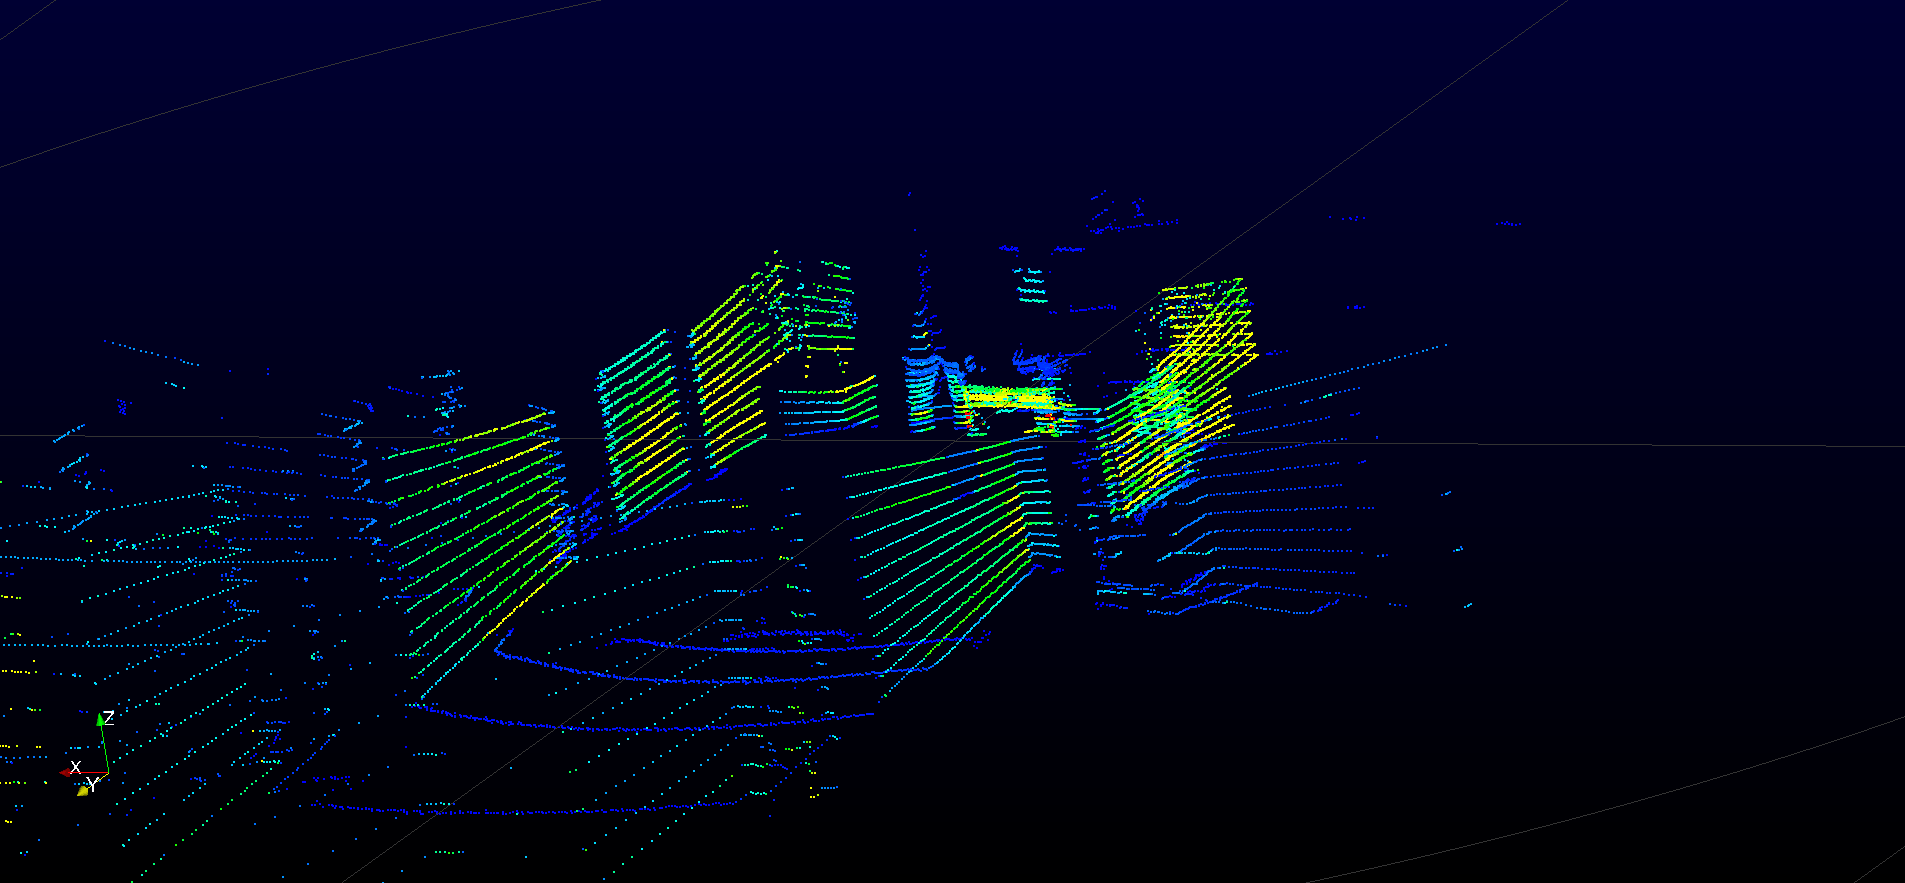
\includegraphics[width=\linewidth]{Figures/lidar_preview.png}
\caption{Zobrazení dat z modelu VLP-16 pomocí softwaru VeloView. }
\label{fig:lidarexample}
\end{figure}

Cílem tohoto projektu je vytvořit nástroj ve webovém rozhraní, který bude sloužit pro označování objektů v LIDARových i obrazových datech. Tyto data budou sloužit jako vstup pro budoucí analýzu dat. Projekt bude obsahovat i serverovou část pro implementaci přijímání a odesílání LIDARových dat a obrázků prostředí. Serverová část nám nejdříve pošle data, která ve webovém prostředí zobrazíme. Na tomto prostředí bude naimplementované označování objektů, kde uživatel označí objekt, a pak všechna označená data posíláme na serverovou část pro uložení. Na serverovou část se bude posílat i snímek bez LIDARových dat. Data na serveru budou použita pro následovnou analýzu obrazu a vizualizační nástroj bude sloužit i k opětovnému přehrání označených dat. Snímek bude sloužit pro lepší představu o tom, o jaký objekt se jedná, protože u LIDARových dat to nemusí být vždy přesné. 
% zeptat se využití dat


\section{LIDAR}
V této kapitole si vysvětlíme princip fungování LIDARu, ukládání dat a přesněji představíme námi použitý model. Také si vysvětlíme pojmy, které budeme používat v dalších kapitolách.
\subsection{Princip fungování LIDARu}
V úvodu jsme Vám krátce představili, co je to LIDAR a jak fuguje. Pojďme se nyní podívat na fyzické fungování modelu VLP-16, se kterým jsme pracovali.  
Základní složkou, kterou LIDAR využívá a počítá s ní je světlo a rychlost světla. LIDAR střílí světelné paprsky, které rychlostí světla letí k cíli. Část tohoto světelného paprsku se po nárazu s objektem odrazí, a putuje zpět stejnou rychlostí ke zdroji paprsku, kde paprsek zachytí senzor. Po dobu celého tohoto procesu je zaznamenáván čas, takzvaný čas letu. Z těchto informací dostáváme rovnici \eqref{eq:eq0}, která popisuje jak LIDAR počítá vzdálenost bodu. Zkratka \texttt{s} značí vzdálenost, \texttt{c} rychlost světla a \texttt{t} čas.

\begin{equation}
		s = \frac{\left ( c \cdot t \right)}{2} 
\label{eq:eq0}
\end{equation}

Pro představu, některá zařízení dokáží vystřelit až \num{150000} paprsků za sekundu. Vlnová délka se liší v závislosti na vzdálenosti a přesnosti. Pohybuje se v rozmezí 600-1000 \si{\nano\metre}. Čím nižší vlnová délka, tím je světlo méně pohlcováno vodou, ale za cenu vzdálenosti, na které je paprsek přesný. Z těchto poznatků je zřejmé, že stojí zvážit vlnovou délku v závislosti na využití. 
Každý LIDAR má určitý počet kanálů, v rozmezí 8-128 kanálů laserových paprsků. S rostoucím počtem kanálů roste i rozlišení a větší přesnost mapovaného prostředí. Toto rozlišení je klíčová vlastnost, která je nezbytná v samořídících autech. Důvodem je víc informací o aktuálním prostředí, rychlejší a častější sběr informací. Samořídící auto, které je vybavené třicetidvou kanálovým LIDARem může jet bezpečně \num{56} \si{\km\per\hour}. Auto s stodvacetiosmi kanálovým LIDARem může jet rychlostí až \num{104} \si{\km\per\hour}. S rostoucí rychlostí potřebují mít senzory více kanálů.

\subsection{Model VLP-16}
Model VLP-16 byl využit při sběru dat pro naše účely. Zde je pár z jeho typických vlastností. Tento model má 16 kanálů. Sběr jedné kompletní odpalovací sekvence trvá \num{55,296} $\mu$s. Laser tohoto modelu pracuje na vlnové délce \num{905} \si{\nano\metre}. Mapa kanálů a úhlů, pod kterými operují paprsky laseru zmíněné v tabulce \ref{tab:tab1}. Díky nízké vlnové délce laseru má nízkou spotřebu energie. Funkční vzdálenost je až \num{100} metrů. LIDAR má horizontální zorné pole $360^ \circ$ a vertikální zorné pole $\pm 30^\circ$. Těmito vlastnostmi dokáže  model získat dostatek kvalitních dat o objektech okolo sebe. Navíc váží pouze \num{830} gramů s velmi nízkou spotřebou elektické energie. V tomto modelu je zaintegrován webový server pro jednoduchý monitoring a konfiguraci od výrobce. Tento model je specializován pro přenos dat po síti. Ethernetové připojení dokáže posílat data rychlostí až \SI{100}{MBps}. Je schopen ukládat záznamy paketů posílané přes ethernet. Jaká data a v jakém formátu jsou obsažena v jednotlivých UDP paketech se dozvíme v kapitole \ref{secref:secref1}.



\subsection{Základní pojmy}\label{sec:sec1}
V této kapitole najdeme nejdůležitější informace, nutné k porozumění LIDARu. Laserovému paprsku se se zvětšující vzdáleností zvětšuje velikost. Velikost rozptylu je \num{3} \si{\milli\radian}. Tímto rozptylem se zároveň snižuje přesnost bodu na větší vzdálenost.

\subsection{Odpalovací sekvence}
Odpalovací sekvencí se označuje vždy čas, kdy byly vyslány paprsky laseru do všech možných úhlů v jednom azimutu. 
Jaké úhly a jaké množství paprsků přesně má model LIDARu? Například model VLP-16 má 16 úhlů, do kterých se paprsky vysílají. 

\subsection{Režimy vrácení dat}\label{sec:sec2}
LIDAR je schopný pracovat ve dvou režimech. Nejdříve si ale budeme muset vysvětlit, jaká data nám LIDAR může vrátit. Při putování paprsku je možné, že paprsek světla narazí do prvního objektu, tomuto bodu dotyku budeme říkat bod A. Tento objekt bude průhledný. Protože je objekt průhledný, tak nepohltí a neodrazí celý paprsek zpět. Z prvního střetu je část paprsku odražena zpět k LIDARu. Paprsek po průchodu prvním objektem pokračuje dál a narazí na jiný objekt, například zeď. Místu střetu se zdí budeme říkat bod B. Po tomto střetu se zbytek světelného paprsku odrazí zpět k senzoru. Nyní máme bod A a bod B, které LIDAR zaznamenal. Záleží na nastavení režimu, který rozhodne zda uloží oba body nebo jen jeden. Bod A se nám vrátí k sensoru jako první. Díky průhlednosti materiálu se část paprsku vrátí a část projde dál. Bod, který LIDAR zaznamenal se vrátí jako nejsilnější vrácený bod, v angličtině nazvaný jako \uv{strongest return}. Zbytek paprsku, který se odrazil od zdi, v našem případě bod B, nazýváme poslední vrácený bod, v původním znění jako \uv{last return}. Toto jsou dva typy bodů, které je LIDAR schopen vrátit.  

%Vrácená data ze senzoru se dělí na dva různé typy. Oba z níže uvedených typů určují, co se s paprskem dělo za jeho cesty k zasaženému objektu. Tyto typy jsou zásadní ve zobrazování dat. 
	\begin{itemize}
		\item Návrat dvou (Dual return)
		\item Návrat jednoho (Single return)
	\end{itemize}
	
Režim vrácení dat si uživatel může při konfiguraci LIDARu nastavit. Režim návrat dvou nám zařizuje vrácení nejsilnějšího  i posledního vráceného bodu. Tato konfigurace nám zaručí přesnější obraz prostředí. Na druhou stranu se pro jeden kompletní obraz posílají \num{2} rámce s daty. K ukládání dat do rámců se dozvíme více v sekci \ref{secref:secref1}. Tímto zapříčiníme, že doba celkového obrazu se zdvojnásobí. Tento režim se používá převážně k mapování terénů. Zaznamená vegetaci(druhý nejsilnější bod) a samotný terén(nejsilnější bod).

Návrat jednoho, jak už název vypovídá, ukládá pouze jeden druh vrácených dat. Uživatel si při konfiguraci LIDARu může vybrat, jestli ho zajímá poslední vrácený nebo nejsilnější vrácený. Tento režim je dvojnásobně rychlejší než režim návratu dvou a používá se v automobilovém průmyslu, kdy je potřeba rychlost. Proto se většinou nastavuje tento režim s nastavením vrať nejsilnějšího. Nejčastěji je potřeba vrátit pevný objekt, aby systém mohl nasimulovat překážky, na které během provozu může narazit. Pevný objekt bývá v převážné většině nejsilnější vrácený bod. 

\subsection{Vertikální úhly a kanály}
V této části budu tyto úhly ukazovat na modelu VLP-16, ale princip zůstane stejný. Jediný rozdíl bude v počtu laserů a velikosti úhlů. Model VLP-16 má šestnáct kanálů, kde každý kanál má svůj vlastní paprsek laseru. Každý paprsek v laseru má svůj vlastní úhel. Data uložená v datovém bloku jsou indexována podle čísel kanálů.

% add centering for table
\begin{table}[!htbp]
\centering
\caption{Mapa kanálů modelu VLP-16 i s vertikálními úhly.}
\label{tab:tab1}
\begin{tabular}{|c|r|}
\hline
Kanály & Vertikální úhly	\\
\hline
0 &   $-15^\circ$   \\
1 &   $1^\circ$	  \\
2 &   $-13^\circ$  \\
3 &   $-3^\circ$   \\
4 &   $-11^\circ$  \\
5 &   $5^\circ$    \\
6 &   $-9^\circ$   \\
7 &   $7^\circ$    \\
8 &   $-7^\circ$   \\
9 &   $9^\circ$    \\
10 &  $-5^\circ$  \\
11 &  $11^\circ$  \\
12 &  $-3^\circ$  \\
13 &  $13^\circ$  \\
14 &  $-1^\circ$  \\
15 &  $15^\circ$  \\
\hline
\end{tabular}
\end{table}

Vertikální úhly jsou určeny vzhledem k vodorovné ploše procházející středem LIDARového senzoru. Každý vrácený bod v datovém bloku je uložen pod číslem kanálu. 
 
\subsection{Mrak bodů}
V angličtině známý jako \uv{Point cloud}. Jak název již napovídá, je to množina bodů v prostoru. Mrak bodů bývá vytvořen 3D skenery jako je LIDAR. Tento pojem se používá při vizualizaci těchto dat, protože když se podíváme na výsledek tak vážně vidíme oblak bodů. Tato práce je o vizualizaci těchto bodů v libovolném webovém frameworku a následnou selekci.

%\subsection{Data blok}


\subsection{Data}\label{secref:secref1}
Každý model ukládá data v různých formátech. Data jsou uložená v paketu, který je složen z jednoho až n datových bloků. Každý z těchto datových bloků je složen z jedné až n dat z odpalovacích sekvencí, které jsou uložené pod číslem kanálu. Tato část bude specifičtěji zaměřená na model VLP-16. Celý paket má velikost \num{1248} bytů. Těchto \num{1248} bytů je rozděleno do hlavičky paketu, datových bloků, timestampu a factory. Hlavička paketu má velikost \num{42} bytů, je důležitá pro internetovou komunikaci pomocí TCP/IP protokolu. Následuje \num{12} datových bloků. Každý z těchto datových bloků má velikost \num{100} bytů. Skládá se z označujících dvou bytů, které označují začátek nového datového bloku, dvou bytů velikosti azimutu a z \num{96} bytů čistých dat. Tyto data mají v sobě dvě odpalovací frekvence, kde jedna odpalovací frekvence má \num{16} kanálů. Dohromady máme \num{32} kanálů, kde každý kanál se skládá ze \num{2} bytů vzdálenosti a jednoho bytu reflektivity. Celkem máme 32(2+1), to je \num{96} bytů plus \num{4} byty. Dohromady máme \num{100} bytů, které nám dávají jeden kompletní datový blok. Azimut, označený na začátku datového bloku, je pouze pro první odpalovací frekvenci. Azimut pro druhou odpalovací frekvenci není explicitně napsán v datovém bloku, ale může být vypočten přičtením jedničky. Stále nám zbývá posledních 6 bytů do \num{1248} bytů. V prvních \num{4} bytech máme uložené časové razítko, které je synchronizováno s GPS systémem. A v posledních dvou bytech je uložené tovární nastavení. V prvním z těchto bytů je uložen režim vrácení dat, již zmíněno v kapitole \ref{sec:sec2}, a v posledním bytu je uloženo označení modelu. Hodnoty a význam těchto bytů uvidíme lépe na obrázku \ref{fig:packet}.

%add citation
\begin{figure}[H]
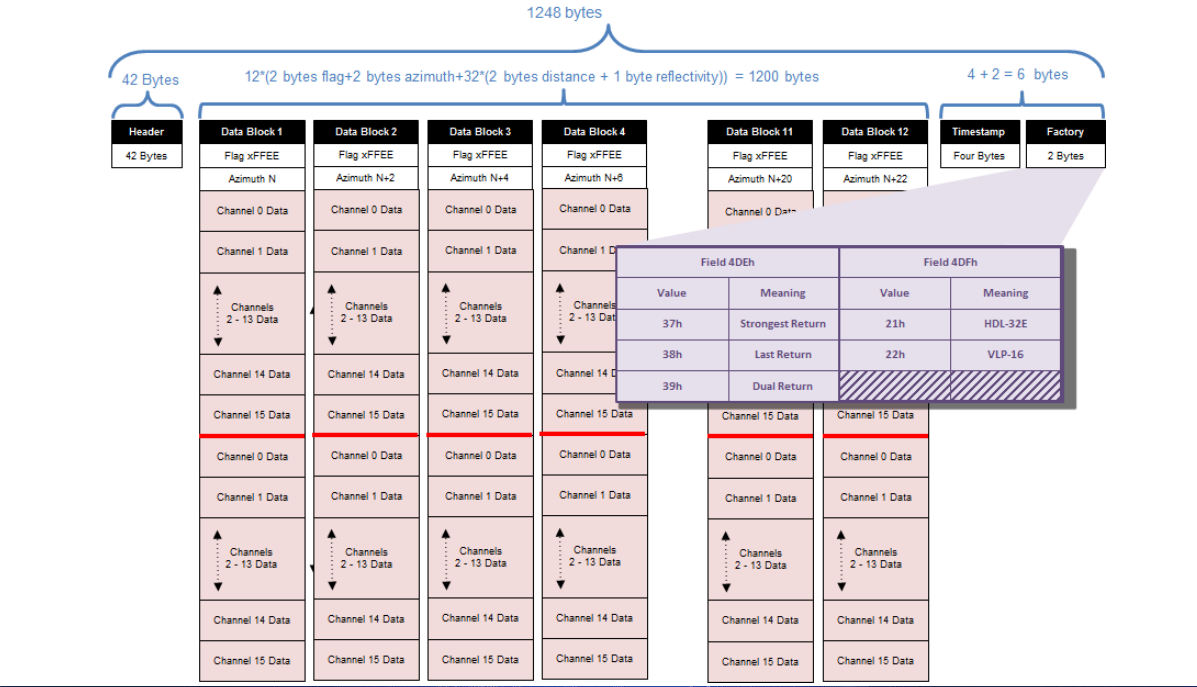
\includegraphics[width=\linewidth]{Figures/packet.png}
\caption{ Paket modelu VLP-16 \cite{packet}. }
\label{fig:packet}
\end{figure}

Značka \texttt{xFFEE} na začátku každého datového bloku značí zahájení nového datového bloku. Tato hodnota je určená výrobcem a je neměnná. \texttt{Factory}, tovární nastavení na konci paketu, s hodnotou 37 hexadecimálně označuje, že LIDAR je nastaven v režimu vrácení jednoho s nastavením vrať nejsilnější bod. Hodnota \num{38} hexadecimálně označuje také režim vrácení jednoho, ale vrací poslední vrácený bod. Poslední možnost s hodnotou \num{39} hexadecimálně znamená režim vrácení dvou. Poslední byte označuje model, ze kterého je tento paket.

Obsah paketu se liší v obsahu při režimu vrácení jednoho a vrácení dvou. Při režimu vrácení dvou se posílají stejné pakety s rozdílem, že se posílají párové datové bloky. Párovým blokem jsou myšleny dva datové bloky paketu, které obsahují odpalovací sekvence se stejným azimutem. Na obrázku \ref{fig:packet2} můžeme vidět dva databloky. Každý z nich obsahuje dvě odpalovací sekvence. Tyto dva databloky mají stejný azimut. První i druhý datablok obsahují stejný azimut odpalovacích sekvencí, ale liší se typem vrácených dat. První z páru vždy obsahuje hodnotu posledního vráceného bodu, druhý datový blok obsahuje hodnotu nejsilnějšího vráceného bodu. 
 
%add citation
\begin{figure}[H]
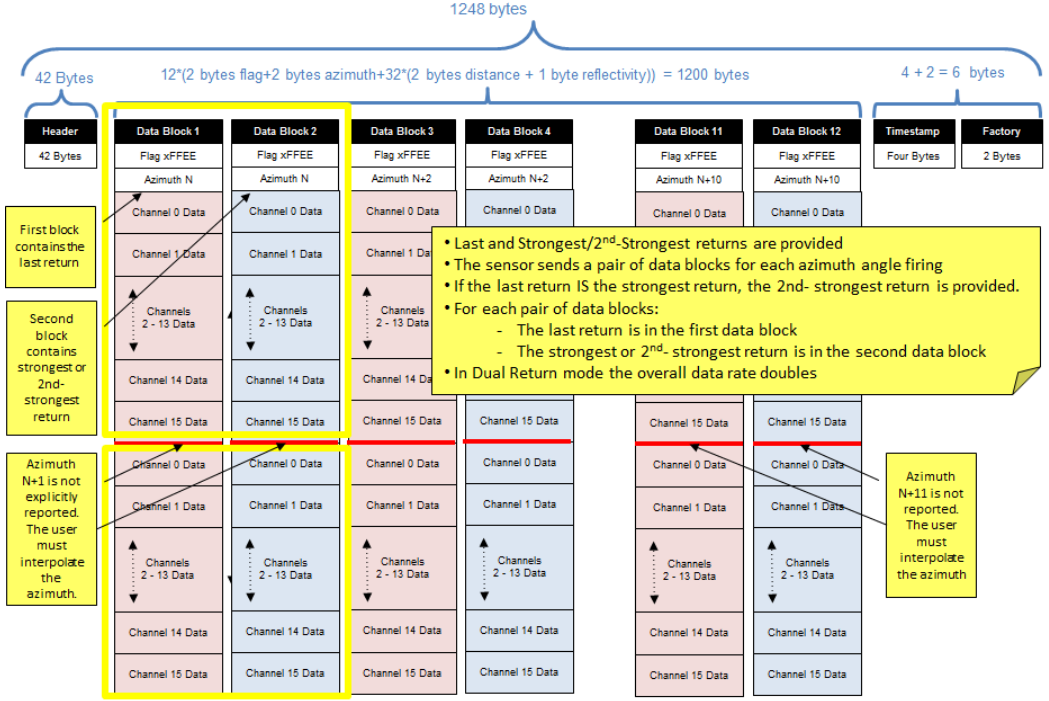
\includegraphics[width=\linewidth]{Figures/paket-dual.png}
\caption{ Paket modelu VLP-16 v režimu vrácení dvou \cite{packet}. }
\label{fig:packet2}
\end{figure}

% přidat python script do veloview
\subsection{Předzpracování dat}\label{secref:predzpracref1}
Předzpracování dat závisí na tom, zda chceme provádět přenos dat v realném čase ke zpracování, nebo ukládat pakety dat do souborů s příponou \texttt{.pcap}. Přenos dat v reálném čase se využívá v autonomních automobilech, kde automobil můsí reagovat na překážky. My nebudeme potřebovat komunikaci a vizualizaci v reálném čase. Účel budovaného systému bude hlavně k vizualizaci LIDARových dat a následnému označování určitých částí mraku bodů, který budeme vracet na serverovou část k úložení snímku vybrané části i všech LIDARových bodů z označené oblasti. 
Data proto nezískáváme z aktivní komunikace LIDARu se zařízením, ale z \texttt{pcap} souborů vytvořených LIDARem. \texttt{Pcap} soubor je záznam komunikace přes TCP/IP protokol. Tento soubor je složen z mnoha paketů \ref{secref:secref1}. K vizualizaci dat z \texttt{pcap} souboru nejdříve musíme extrahovat informace, které jsou uvnitř jednotlivých paketů. Data jsme se rozhodli transformovat rovnou do kartézských souřadnic, abych předešel zbytečným a velmi komplikovaným výpočtům na straně uživatele. K tomuto účelu jsme použili Python konzoli v programu VeloView. Hlavním důvodem využití této konzole bylo přístupné Python rozhraní pro práci s \texttt{pcap} soubory. Zmíněné rozhraní používá knihovnu napsanou v jazyce C++, aby zpracování bylo co nejrychlejší. Tato knihovna je specificky napsána pro práci s LIDARem a \texttt{pcap} soubory, proto jsme vytvořili jednoduchý script v Pythonu, který využívá již zmíněné rozhraní a přetransformuje nám \texttt{pcap} soubor na neznámý počet JSON souborů. Každý JSON soubor obsahuje jeden kompletní mrak bodů.

\lstinputlisting[language=python,caption=Python script pro transformaci \texttt{pcap} souborů na JSON soubory.]{SourceCodes/transformdata.py}

Tento script spouštíme v Python konzoli programu VeloView po načtení \texttt{pcap} souboru. Příkaz \texttt{vv.gotoNext()} nás přesune na další ze zmapovaných mraků bodů. V proměnné \texttt{cloudinfo} máme uložený aktuální snímek mraku bodů, který má uživatel zobrazen a všechna možná dostupná data, která byla v paketech uložena i s metadaty. Proměnná \texttt{points} nám vrátí pole všech bodů aktuálního mraku bodů. Každý tento vrácený bod obsahuje trojici čísel, která odpovídá kartézským souřadnicím v prostoru. Proměnná \texttt{data} je slovník, do kterého v cyklu ukládáme námi potřebná data. Slovník je specifický tím, že se do něj ukládá klíč a na daný klíč je navázaná hodnota, v našem případě klíč je číslo bodu a k tomu navazující hodnota z proměnné \texttt{points} na indexu klíče. Po ukončení všech iterací cyklu vytvoříme soubor a pomocí externí knihovny \texttt{json}, který jsme si na začátku scriptu importovali, vytvoříme ze slovníku JSON řetězec a uložíme ho do souboru. Každý soubor začíná prefixem \texttt{LidarData\_X}, kde X je index aktuálního mraku bodů. Po spuštění tohoto scriptu máme všechna data, která potřebujeme na vizualizaci mraku bodů a následné práce s ním. 




\section{Vizualizace}
Tato část je určena vizualizaci. V této kapitole si ukážeme, jak jsme postupovali při vývoji systému. Od procesu výběru technologií a frameworků až po principy vykreslování. Ze zadání je zřejmé, že vizualizace dat musí probíhat v prohlížeči na straně uživatele a musí být zobrazená ve 3D. V serverové části budeme mít možnost si uložit námi vybraná data popřípadě obrázky.

\subsection{Výběr technologií} 
Na straně uživatele používáme programovací jazyk JavaScript. K těmto účelům bylo vytvořené JavaScriptové rozhraní pro použití WebGL, které využívá rozhraní OpenGL. OpenGL je abstraktní rozhraní pro práci s grafikou. Implementace OpenGL jsou vytvořeny pro všechny platformy a naprogramovány na rychlejších jazycích, pracují přímo s grafickou kartou pro vysokou výpočetní rychlost. Knihovna, kterou jsme si vybrali je Three.js. Three.js je knihovna, která detekuje verzi prohlížeče a použije nejnovější technologie a nejnovější implementace JavaScriptu, které jsou prohlížečem možné použít. Hlavními důvody, proč jsme použili tuto 3D knihovnu, byla její rozsáhlá a detailně zpracovaná dokumentace. 
V serverové části jsme se rozhodli použít programovací jazyk Java. Bude mít za úkol posílat body mraku bodů na stranu uživatele a zpracovat, nebo uložit data odeslaná uživatelem. Pro vytvoření webové aplikace jsme využili knihovnu \texttt{Spring Boot}. Dalším rozšířením je knihovna Thymeleaf  pro dynamické renderování \texttt{HTML} na straně serveru. Již zmíněné technologie jsou nedílnou součástí praktické části. Jako bundler statických prvků a minifikaci JavaScriptu jsme použili nástroj zvaný \texttt{Webpack}. Jeho výhodou je jednoduchá konfigurace a používání. Bundler nám spojí všechny potřebné použité javascript soubory do jednoho zminifikovaného souboru. Pro ukládání dat použijeme objektově-relační databázový server PostgresSQL, který je zdarma a je připravený na vysoký počet požadavků.
 
\subsection{Alternativní knihovny} Je mnoho alternativních knihoven, které jsme mohli použít. Ukážeme si pár z nich. Za zmínku stojí Babylon.js. Tato knihovna se používá na vytváření her v prohlížeči. Kód z Babylon.js je možné exportovat do Unity 3D herního enginu. Zaměřuje se tedy více na kolize, události, rendering a vyhlazování. Oba dva jsou v tuto chvíli nejlepšími 3D JavaScriptovými knihovnami s open source licencí. Alternativou Webpack bundleru je \texttt{Rollup}. Konfigurací se velmi podobá \texttt{Webpack} bundleru. Je jen o zanedbatelnou dobu pomalejší. Na straně serveru jsme mohli použít mnoho různých alternativ, protože požadavek od serveru je odpovídat a přijímat žádosti o data a posílat je uživateli na jeho rozhraní, přijímat označená data z uživatelského rozhraní a ukládat je na straně serveru k budoucí analýze. Další možností byla webová aplikační knihovna \texttt{Django} s programovacím jazykem Python. Tato kombinace je velmi dobrá pro rychlý vývoj jednoduchých aplikací. Další alternativou bylo PHP s některým z frameworků, jako je například Laravel. Neměli jsme žádné specifické požadavky od systému, ve kterých bychom mohli říct, že využijeme určitý programovací jazyk, protože by byl pro tuto problematiku lepší. Požadavky od naší serverové části by efektivně zvládlo mnoho jazyků. Nelze tedy z našich požadavků vybrat jen jeden jazyk a říct, že pro nás bude nejlepší. Pro databázový server jsme měli mnoho možností. Jedním z mnoha je \texttt{MySQL}. Tento databázový server je velmi rychlý i ve velkém množství čtecích operací. Je také úspornější na místo v paměti, ale za cenu problému s konkurencí. Pro náš systém jsme potřebovali databázový systém, který bude efektivně číst a psát větší množství dat.


\subsection{Základy knihovny Three.js} Abychom mohli pomocí knihovny Three.js cokoliv zobrazit, tak k tomu potřebujeme tři nezbytné a základní věci, bez kterých bychom se neobešli. Těmito třemi základními věcmi jsou scéna, kamera a renderer. Scéna je virtuální trojrozměrný prostor, do kterého přidáváme objekty. Kamera nám zařizuje projekci objektů na 2D obrazovku, jaký typ projekce záleží na kameře. Poslední a nejdůležitější částí je renderer. Renderer nám zařizuje vykreslení scény z pohledu kamery, popřípadě více kamer. Stále nám však tyto prvky nemají co zobrazit, nejdříve si musíme vytvořit nějaké objekty, které můžeme přidat do scény. Každý objekt musí mít pozici, na kterou ji přidáváme do scény. Scéna v \texttt{Three.js} má souřadnicový systém pravotočivý. Když si vezmeme pravou ruku a dáme ji dlaní před sebe, tak osu \texttt{x} představuje palec, ukazováček směřující vzhůru je osa \texttt{y} a pokrčený  prostředníček směřující k tělu je osa \texttt{z}.
% maybe add more how camera works frustum etc.

\subsection{Vytváření objektů v Three.js}\label{secref:secref6}
K vytvoření každého objektu potřebujeme množinu vrcholů, stěn a materiálů ve WebGL. Three.js má již jednoduché rozhraní, které nám dovoluje vytvářet různé objekty, bez znalostí knihovny WebGL. Knihovná má již vyřešené vytváření základních 3D geometrických objektů, jako je krychle, koule, křivky a mnoho dalších. Zde je ukázka vytvoření koule o poloměru \num{0,005}. 

\lstinputlisting[language=JavaScript,caption=Vytvoření koule za pomoci knihovny Three.js]{SourceCodes/threeJSSphere.js}

První potřebujeme vrcholy a stěny. O to se nám postará \texttt{THREE.SphereGeometry}, který jako první parametr bere průměr koule, druhý parametr je počet segmentů na šířku a třetí počet segmentů na výšku. Čím více segmentů daná koule má, tím je přesnější a kulatější. Rozdíly můžeme vidět na obrázku \ref{fig:spheres}. Počty segmentů jsou shora i zdola omezeny. Maximum je \num{32} u výšky i šířky a minimum se liší. U výšky je minimum \num{2} a u šířky je minimum \num{3}.

\begin{figure}[H]
    \centering
    \subfloat[Pět segmentů na výšku i šířku]{{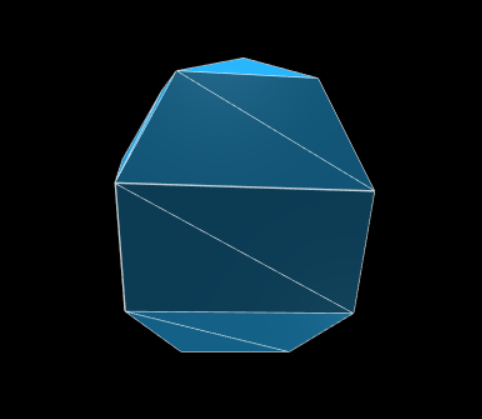
\includegraphics[width=5cm]{Figures/sphere1.png} }}
    \qquad
    \subfloat[Třicetdva segmentů na výšku i šířku]{{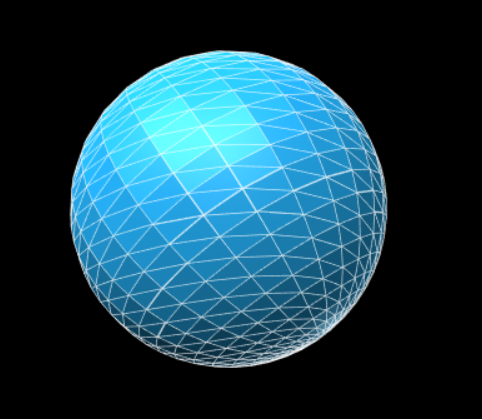
\includegraphics[width=5cm]{Figures/sphere2.png} }}
    \caption{Rozdíly v počtu segmentů}%
    \label{fig:spheres}%
\end{figure}

S narůstajícím počtem segmentů jsou nároky na GPU vyšší, protože musí vykreslit více vrcholů a hran koule. Proto jsme v projektu použíli malý počet segmentů na výšku i šířku koulí \num{5}. Když si uvědomíme, že každé vykreslení mraku bodů má \num{25000} takových koulí, tak chceme nároky na GPU co nejnižší.
Dále potřebujeme ještě materiál, který nám vyplní všechny stěny a vrcholy. Je hodně různých druhů materiálů. Každý materiál má své specifické vlastnosti, jak se zobrazuje ve světle. Tato vlastnost \texttt{THREE.MeshLambertMaterial} v kombinaci se světlem nám velmi pomůže rozlišit jednotlivé koule (LIDARové body) od sebe. Kdybychom použili materiál \texttt{THREE.Basic}, tak bychom nerozeznali jednu kouli od druhé. Na tento materiál nepůsobí světlo, proto ať už bychom se podívali na jakoukoliv část koule, tak by měla konstantní odstín barvy materiálu. Koule by splývaly mezi sebou. Při vytváření nové instance materiálu nesmíme zapomenout přidat barvu do konstruktoru. \texttt{THREE.Mesh} si jako argument požaduje geometrii a materiál, který má vyplnit stěny dané geometrie. Mesh nám vytvoří výsledný objekt, v našem případě kouli. Tento objekt je možné vložit přímo do scény pro zobrazení koncovému uživateli.

\subsection{Konkurenční řešení}
Jedno z konkurenčních řešení je program VeloView. Program VeloView je aplikace na stolní počítač, který slouží pouze k vizualizaci LIDARových dat z LIDARů od firmy Velodyne. Firma Velodyne se specializuje převážně na zlepšení a zdokonalení LIDARů zaměřených na automobilovou část průmyslu. Veloview, narozdíl od našeho vytvářeného systému, není ve webovém rozhraní dostupný odkudkoliv a z jakéhokoliv systému. Dalším rozdílem je, že zobrazuje čistě LIDARová data a nedovoluje nám přidat pozadí, abychom si mohli i graficky představit prostředí, v jakém se pohybujeme. Označování objektů a následný export dat je v obou již zmiňovaných LIDARových nástrojích.
Další alternativou je Python knihovna s názvem Point Processing Toolkit ve zkratce \texttt{PPTK}. Tato knihovna dokáže vizualizovat body v dvojrozměrném, ale i v trojrozměrném prostoru. Dále podporuje selekci bodů v prostoru přes uživatelské rozhraní, stejně jako program VeloView. Avšak narozdíl od programu VeloView, \texttt{PPTK} data pouze vizualizuje, proto potřebuje data určující pozici v prostoru. VeloView používá data přímo z výstupních souborů, které generuje LIDAR. Stejně jako VeloView je možné tento program použít pouze na počítačích a bez možného přidání snímku do pozadí projekce.


% add kamera?

\subsection{Princip fungování kamery}\label{secref:secref16}
Kamera nám vytváří perspektivní projekci na scénu. Než si vysvětlíme, jak funguje perspektivní projekce, tak si musíme vysvětlit, na jakém principu pracuje kamera. Perspektivní kamera nám zachycuje scénu pohledem oka. Zóna zachycení kamery je specifikována jako frustum. Frustum je složeno z šesti rovin, které dělí prostor. Uvnitř frustumu je zachycena část scény, kterou chceme kamerou zobrazit. Frustum se skládá z šesti rovin: horní, spodní, nalevo, napravo a dvě roviny vpřed a v dálce. Úhlu mezi horní a dolní rovinou se říká horizontální field of view, zkráceně FOV. Tento úhel bývá v rozmezí $30^\circ-60^\circ$. Přední rovina ohraničená dalšími rovinami je naše obrazovka, do této roviny se provede projekce všeho, co je ve frustumu. 

\begin{figure}[H]
\centering
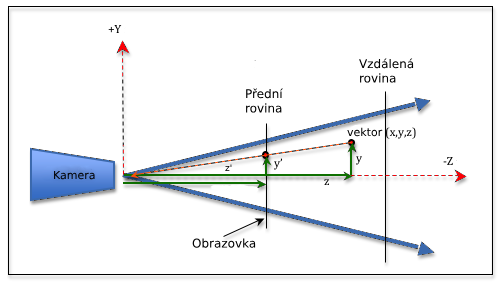
\includegraphics[width=\linewidth]{Figures/perspectiveProjection.png}
\caption{Perspektivní projekce kamery \cite{learnwebgl}. }
\label{fig:perspectiveProjection}
\end{figure} 

Jak můžeme vidět na obrázku, když chceme promítnout bod na přední rovinu (naše obrazovka), tak vektor ze středu kamery k vrcholu objektu musí protnout přední rovinu. Bod střetu tohoto vektoru s rovinou je perspektivní projekce tohoto bodu na naši obrazovku. Takto je to provedeno se všemi hranami a vrcholy všech objektů. Tímto promítnutím na plátno zůstává zachovaný poměr $\frac{y'}{z'}=\frac{y}{z}$. 


Pro zjišťování obrysů ve scéně za našim kurzorem budeme používat Ray-tracing algoritmus. Ray-tracing, jak už z názvu vyplívá, bude sledovat paprsek, který vychází ze středu kamery přes promítací rovinu a zachytí všechny stěny geometrie po jeho trase. Při získání geometrie, kterou protnul si zjistí, o jaký objekt se jedná. Ukážeme si to na obrázku \ref{fig:perspectiveProjection}. Paprsek nám vznikne ve středu kamery a protíná určité místo promítací roviny. Tímto se snažíme najít jakýkoliv objekt, který za tímto místem je. Používáme implementaci tohoto algoritmu ve třídě \texttt{raycaster}.


\section{Implementace}
V této kapitole najdeme postup a implementaci systému od úplného začátku až do konce. Začneme na serveru od základní funkcionality až po datový model, pak se přesuneme na vizualizaci a selekci i s odesíláním dat na straně uživatele.


\subsection{REST API} 
REST API je rozhraní na straně serveru, které za pomoci HTTP požadavků provádí akce s daty. Cílem je vytvořit akce na url adresy pro získání/uložení LIDARových dat. Akce musí být parametrizovatelné, abychom věděli, jaká data máme poskytnout, popřípadě uložit. Nejdříve potřebujeme mít nějaká lidarová data a snímky z přední a zadní strany jízdy. Tato data musíme mít uložené na serveru, přesněji v databázi, abychom je mohli poskytovat uživateli. Dále uživatel si bude moci vybírat určité části lidarového mraku bodů s obrazovými daty, a proto je budeme muset uložit. Dále ještě musíme poskytnout již zmíněné selekce k znovuzobrazení. Tyto služby budeme pomocí \texttt{REST API} poskytnout, aby mohla aplikace na straně uživatele komunikovat se serverem.


\subsection{Datový model} 
Důležitou částí je datový model našeho informačního systému. Model si rozdělíme podle chtěných požadavků od serveru, ukládání selekcí objektů a získávání všech možných dat z jednoho mraku bodů. Na obrázku \ref{fig:datamodel} můžeme vidět rozdělení těchto požadavků zobrazených UML diagramem. Tabulka \texttt{main\_menu\_storage} obsahuje všechny unikátní výjezdy s LIDAR zařízením. Každý mrak bodů je uložen na samostatném řádku, tabulka \texttt{raw\_data\_store}, s přímým odkazem na to, v jaké jízdě byl zaznamenán a odkazem na další tabulku \texttt{raw\_data\_pictures}. V této tabulce jsou uloženy odkazy ke snímkům na disku z přední a zadní strany vozidla. Tyto zmíněné tabulky jsou potřebné k posílání dat na stranu uživatele za účelem vizualizace. Druhou částí je ukládání selekce specifických objektů, které si uživatel vybral. V tabulce \texttt{selected\_data\_parts} jsou uložené všechny body dané selekce s informací, ze kterého mraku bodů byla vytvořena. Jsou zde uloženy ještě další informace. Mezi tyto informace patří jméno objektu v selekci, tabulka \texttt{selected\_item\_name} a snímek selekce, tabulka \texttt{selected\_item\_pictures}.



\begin{figure}[H]
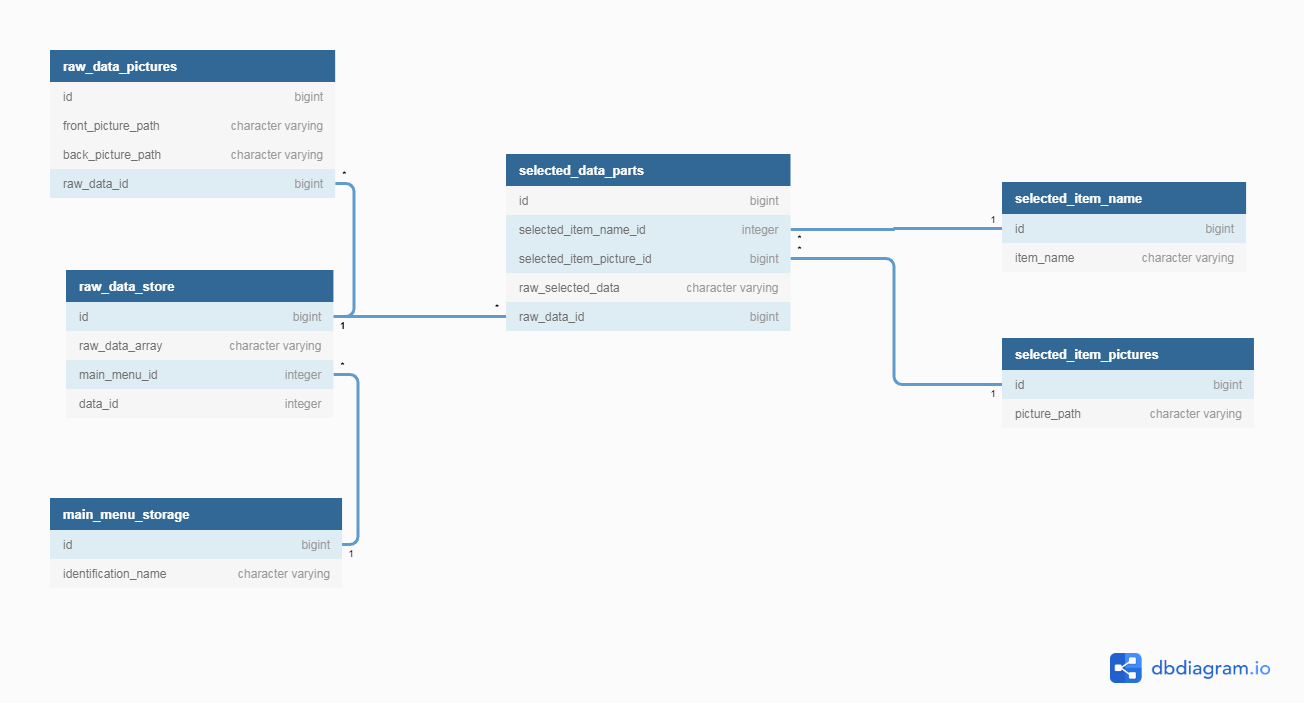
\includegraphics[width=\linewidth]{Figures/dataModel.png}
\caption{Datový model informačního systému. }
\label{fig:datamodel}
\end{figure} 



\subsection{Scéna a kamera} Scéna je náš virtuální prostor, do kterého budeme přidávat LIDARové body. K chtěnému zobrazení této scény potřebujeme ještě kameru a renderer. Kamera nám ohraničuje specifickou část prostoru, kterou nám renderer zobrazí. Tato část prostoru se nazývá kamerové frustum. Renderer nám zajistí, aby se pracovalo pouze s objekty, které leží uvnitř tohoto frustumu. Kamera nám zajistí projekci viz. \ref{secref:secref16}. 

\begin{minipage}{\linewidth} 
\lstinputlisting[language=JavaScript,label={secref:secref17},caption=Vytvoření scény s kamerou a rendererem.]{SourceCodes/mainScene.js} 
\end{minipage} 
V kódu \ref{secref:secref17} vidíme konstruktor a metody \texttt{animate}, \texttt{stopAnimation} a \texttt{onWindowResize}. V konstruktoru vytvoříme virtuální scénu, perspektivní kameru a renderer. Vytvoření je velmi snadné s \texttt{Three.js} knihovnou. Pro náš projekt jsme si vybrali perspektivní kameru, abychom napodobili pohled lidského oka, které zkresluje velikost objektu s rostoucí vzdáleností. Tímto se liší ortografická kamera od perspektivní. K vytvoření kamery potřebujeme nejdříve pár důležitých parametrů. Prvním parametrem je \texttt{field of view}, neboli zorné pole. Tímto číslem určíme úhel ve stupních, který bude mít vertikální úhel kamerového frustumu. Vertikální FOV u běžných kamer jsou v rozmezí $60\circ$ - $110\circ$. Druhým parametrem je poměr stran rámce, do kterého budeme chtít zobrazit naši scénu. V našem případě chceme výsledný rámec přes celou obrazovku prohlížeče, proto \texttt{window.innerWidth / window.innerHeight}. Na základě tohoto parametru si \texttt{Three.js} dopočítá horizontální FOV, aby obraz nebyl zkreslený. Třetí parametr značí vzdálenost, od pozice kamery, k přední stěně pyramidového frustumu. V této vzdálenosti nám vznikne promítací rovina, na kterou se nám promítne scéna a vytvoří nám obraz do našeho rámce v prohlížeči. Poslední parametr značí také vzdálenost, ale k nejvzdálenější stěně kamerového frustumu. Renderer nám zajistí vytvoření výsledného \texttt{HTML canvas} plátna, proto mu musíme určit velikost tohoto plátna. Už stačí jen přidat do objektového modulu dokumentu stránky. To ještě není všechno, stále potřebujeme funkci, která nám bude periodicky vykreslovat aktuální scénu na plátno. K tomuto účelu použijeme metodu \texttt{animate}, která využívá funkci \texttt{requestAnimationFrame}. Tato funkce říká prohlížeči, že chceme provést animaci a specifikovat chování překreslení. Proto do této funkce dáváme jako parametr referenci na funkci \texttt{animate}. Tímto vytvoříme nekonečný cyklus, kde v každé iteraci budeme na rendereru volat metodu \texttt{render}. Ve zmíněném kódu ještě máme vytvořený posluchač na událost \texttt{změna velikosti}, který nám upraví poměr stran kamery a aktualizuje její projekční matici. Dále už jen aktualizuje velikost výsledného plátna. Výsledkem tohoto kódu máme na naší \texttt{HTML} stránce plátno, s pohledem na scénu. Bohužel nic na našem plátně neuvidíme z důvodu, že nemáme žádný objekt ve scéně.



\subsection{Vizualizace LIDARových dat}  
Zakladem našeho informačního systému je uživateli vizualizovat mrak bodů z LIDARového zařízení. K tomuto účelu nejdříve potřebujeme získat data ze serveru. Uživatel musí specifikovat jaká data chce získat, který mrak bodů a z jaké jízdy. Musíme tedy vytvořit uživateli posuvník, kterým se bude orientovat mezi snímky mraku bodů. Tento posuvník bude nabívat hodnot 
$\langle \texttt{0, m}\rangle \subset \mathbb{N}$, kde \texttt{m} je maximálního počtu uložených mraků bodů pro danou jízdu. Pro získání dat mraku bodů si musíme vytvořit požadavek na server. Server nám prostřednictvím \texttt{REST-API} poskytne objekt, který obsahuje \texttt{l} objektů, kde \texttt{l} je množství lidarových bodů v našem mraku. Každý z těchto objektů obsahuje pole s pozicemi v kartézské soustavě souřadnic. Jak jsme získali takto předzpracovaná data najdeme v kapitole \ref{secref:predzpracref1}. Pro získání dat použijeme kód \ref{secref:loaddataref1}.

\lstinputlisting[language=JavaScript,label={secref:loaddataref1},caption=Metoda pro získání LIDARových dat ze serveru.]{SourceCodes/loadDataFromServerAndRenderPoints.js}

Nejdříve si uložíme referenci kontextu do proměnné \texttt{that}, protože později budeme mít kontext \texttt{this} jiný a nedokázali bychom se získat instanční proměnné z naší třídy. Dále specifikujeme jaký požadavek a na jakou url adresu chceme požadavek posílat. Jak můžeme vidět vkládáme do url proměnné z aktuálního kontextu. Budeme totiž chtít specifikovat z jaké jízdy máme brát mraky bodů a zároveň číslo mraku bodů, který uživatel chce vidět. Číslo mraku bodů bude získáno na základě posuvníku. Při zaslání požadavku nikdy přesně nevíme kdy nám server odpoví a kdy nám dorazí data, které jsme chtěli. K tomu nám pomůže funkce \texttt{onreadystatechange}. Ta se spustí vždy, když se změní stav požadavku. My si vytvoříme uvnitř této metody akce, které budeme chtít provést jen když je komunikace ukončena a konečný status požadavku je \texttt{200 OK}. Nasledně jen zpracujeme tělo požadavku z \texttt{JSON} formátu do \texttt{JavaScript} objektu a přejdeme k vykreslení mraku bodů.


\lstinputlisting[language=JavaScript,caption=Metoda pro vykreslení LIDARových dat.]{SourceCodes/renderPointsFromData.js}

\texttt{Three.js} nám umožňuje vytvářet skupiny objektů, které slouží k lepší přehlednosti v kódu. Naši skupinu, \texttt{groupOfPoints}, máme již přiřazenou do scény. Kdykoliv přidáme do této skupiny objekt, automaticky se nám vloží i do naší virtuální scény. K vytvoření meshe potřebujeme dvě věci, geometrii a materiál \ref{secref:secref6}. Protože budeme přepoužívat geometrii a materiál tak si je uložíme do proměnných, ještě před kompletními iteracemi lidarových bodů. V proměnné \texttt{thatPoints} máme data ze serveru. Pak už jen vytvoříme cyklus, který v každé iteraci vytvoří nový mesh objekt a nastavíme mu pozici ve scéně.

\begin{figure}[H]
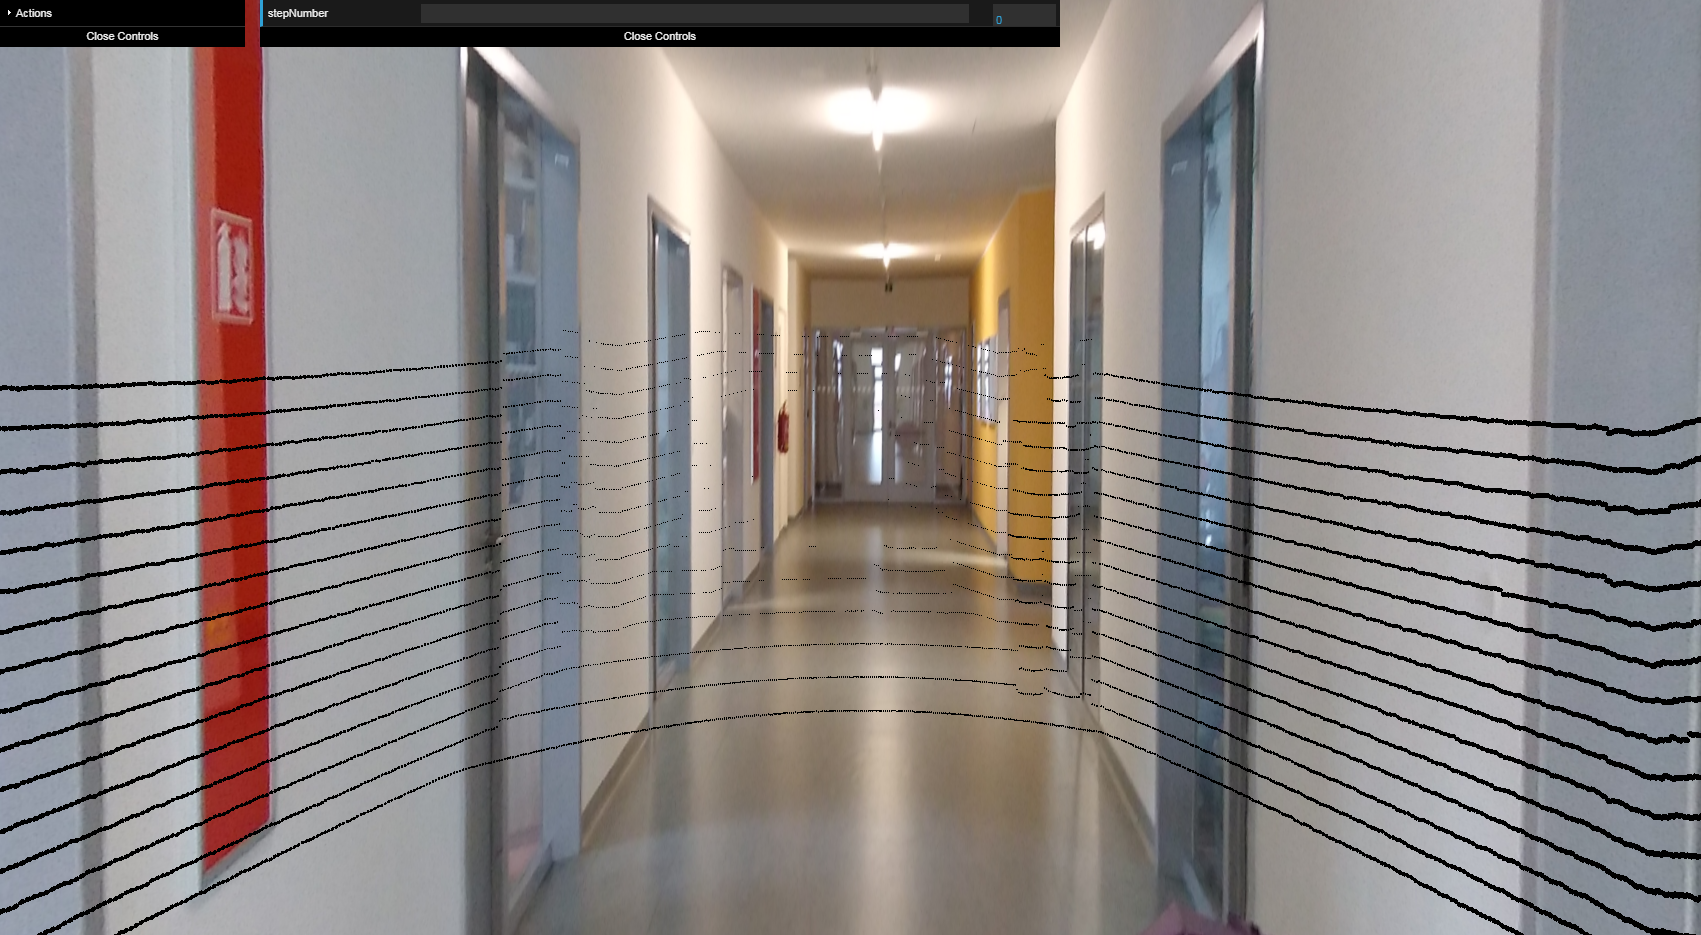
\includegraphics[width=\linewidth]{Figures/sceneWithPoints.png}
\caption{Výsledná vizualizace.}
\label{fig:sceneWithPoints}
\end{figure}
	 

\subsection{Výběr prostoru}\label{secref:secref10}
K označení určité části v prostoru si musíme uvědomit, že na naší obrazovce máme projekci z kamery \ref{secref:secref16}. Tohle je důležité si uvědomit, když budeme chtít z našeho 2D obrazu promítnout náš klik do 3D prostoru. Budeme to potřebovat na vyznačení určité části prostoru. Zde můžeme vidět kód, který nám vytvoří vektor se směrem od kamery k promítací rovině.  

\lstinputlisting[language=JavaScript,label={secref:secref7},caption=Projekce myši do 3D prostoru.]{SourceCodes/mouseProjection.js}

Nejprve musíme vytvořit událost, abychom mohli zjistit pozici kliku. Tato hodnota je vydělena šířkou celého vnitřního okna prohlížeče, to celé vynásobené dvěmi a odečteno jedničkou. Tímto způsobem je vytvořená i \texttt{y} hodnota. Potřebujeme, abychom ve středu obrazovky měli koordinát (0,0), k tomu tato část kódu slouží. Po této kostrukci nám budou hodnoty \texttt{x, y} v intervalu $\left\langle-1,1\right\rangle$. Aby jsme mohli vytvořit vektor v prostoru, tak nám nestačí \texttt{x, y}, proto musíme vytvořit trojrozměrný vector s nově vypočítanými hodnotami \texttt{x} a \texttt{y}. Jako hodnota osy \texttt{z} bude nula. Hodnota z by nám na tomto místě pouze určovala posun od středu kamery k plánu při interních výpočtech. \texttt{THREE.Vector3} má metodu \texttt{unproject} s parametrem typu \texttt{Camera}, vložíme zde naši hlavní perspektivní kameru. Na vektor se aplikuje projekční matice z kamery. Výsledkem se stane vector, který nám ze středu kamery udá směr odpovídající přímce. Na této přímce jsou všechny body, které odpovídají projekci naší akce z obrazovky. Když se podíváme na obrázek \ref{fig:perspectiveProjection}, tak nám pomůže si to lépe představit. Při kliknutí získáme pozici na obrazovce, která na obrázku představuje rovinu blíže kameře a bod ležící na ní. Při provedení výše zmíněného kódu získáme vektor, který nám určí směr v trojrozměrném prostoru. Pak už záleží na nás, v jaké vzdálenosti od kamery požadovanou pozici chceme.

Selekci musíme z dvojrozměrné obrazovky přenést do trojrozměrného prostoru a vizualizovat obrys selekce. Zároveň musí mít obrys všech vyznačených prostorů rotaci takovou, že obrys je natočen kolmo ke středu celého světa. K vytvoření obrysu potřebujeme dva body z obrazovky. Pro první bod použijeme kód \ref{secref:secref7}, a přidáme k němu další část \ref{secref:secref8}.

\lstinputlisting[language=JavaScript,label={secref:secref8},caption=Zvětšení délky vektoru.]{SourceCodes/scalingVector.js}

Nejdříve spočítáme délku vektoru, pak vydělíme číslo tři délkou vektoru. Číslo tři, protože chceme, aby všechny selekce byly v okolí naší pozice maximálně tři jednotky od nás. Později budeme pohybovat naší vyznačenou selekcí okolo naší pozice. Pohybovat jí budeme po kouli, která nás bude obklopovat. A v posledním kroku vynásobíme náš vektor proměnnou \texttt{scalingFactor}. Tímto zajistíme zvětšení vektoru při zachování směru. 

Druhý bod se bude trošku lišit od projekce prvního bodu. 

\lstinputlisting[language=JavaScript,caption=Promítnutí druhého bodu obrysu selekce.]{SourceCodes/secondPoint.js}

Zde se poprvé setkáváme s třídou \texttt{Raycaster}. Tato třída slouží k detekci objektů. Po inicializaci \texttt{raycasteru} musíme namířit na správný směr a nastavit správnou pozici. O to se nám postará metoda \texttt{setFromCamera} se dvěmi vstupními parametry. Prvním je \texttt{THREE.Vector2}, který obsahuje vypočítané údaje pro projekci bodu a druhým parametrem je naše hlavní kamera. Nyní si vytvoříme rovinu z coplanar bodu a normály. Jako coplanar bod využíváme ten, který jsme vytvořili na začátku této podkapitoly. Jako poslední krok řekneme raycasteru, aby vyslal paprsek, který má zkusit protnout rovinu a výsledek uložit do proměnné \texttt{result}.


\begin{minipage}{\linewidth}
\lstinputlisting[language=JavaScript,label={secref:secref9},caption=Vytvoření obrysu selekce.]{SourceCodes/makeBorder.js}  
\end{minipage}

Proměnné \texttt{firstPoint} a \texttt{secondPoint} odpovídají získaným bodům z této podkapitoly. Z těchto trojrozměrných vektorů musíme zjistit délku \texttt{x} a \texttt{y} vytvářeného obdelníku. Tyto vzdálenosti jsou důležité při vytváření našeho obrysového obdelníku. 

\lstinputlisting[language=JavaScript,caption=Použití THREE.Shape k vytvoření obdelníku.]{SourceCodes/create3DLine.js} 

V tomto kódu vytváříme náš vlastní tvar. Postupně, díky délkám stran obdelníku, vytváříme náš vlastní obdelník s pomocí \texttt{THREE.Shape}. Tuto třídu používáme z důvodu jednoduchého rozhraní pro vytvoření geometrie objektu v dvojrozměrném prostoru, která je jednoduše přenesitelná do trojrozměrného prostoru. Po vytvoření našeho obdelníkového tvaru z něj získáme geometrii, a s pomocí materiálu vytvoříme nový objekt typu \texttt{THREE.Line}. Tomuto vrácenému objektu musíme nastavit pozici, protože všechny objekty mají výchozí pozici ve středu scény. Na náš nový tvar musíme ještě aplikovat rotaci podle rotace světa. Důvodem, proč musíme aplikovat rotaci je, že tvar byl vytvořen v dvojrozměrném prostoru a přenesen do trojrozměrného, proto když náš nový tvar přidáme do scény, tak bude vodorovně s osou \texttt{x}, \texttt{y}, ale kolmo na osu \texttt{z} ve všech případech. Nakonec si ještě přidáme do našeho objektu pomocné informace pro budoucí použití a přidáme do skupiny obrysů.

\begin{figure}[H]
\centering
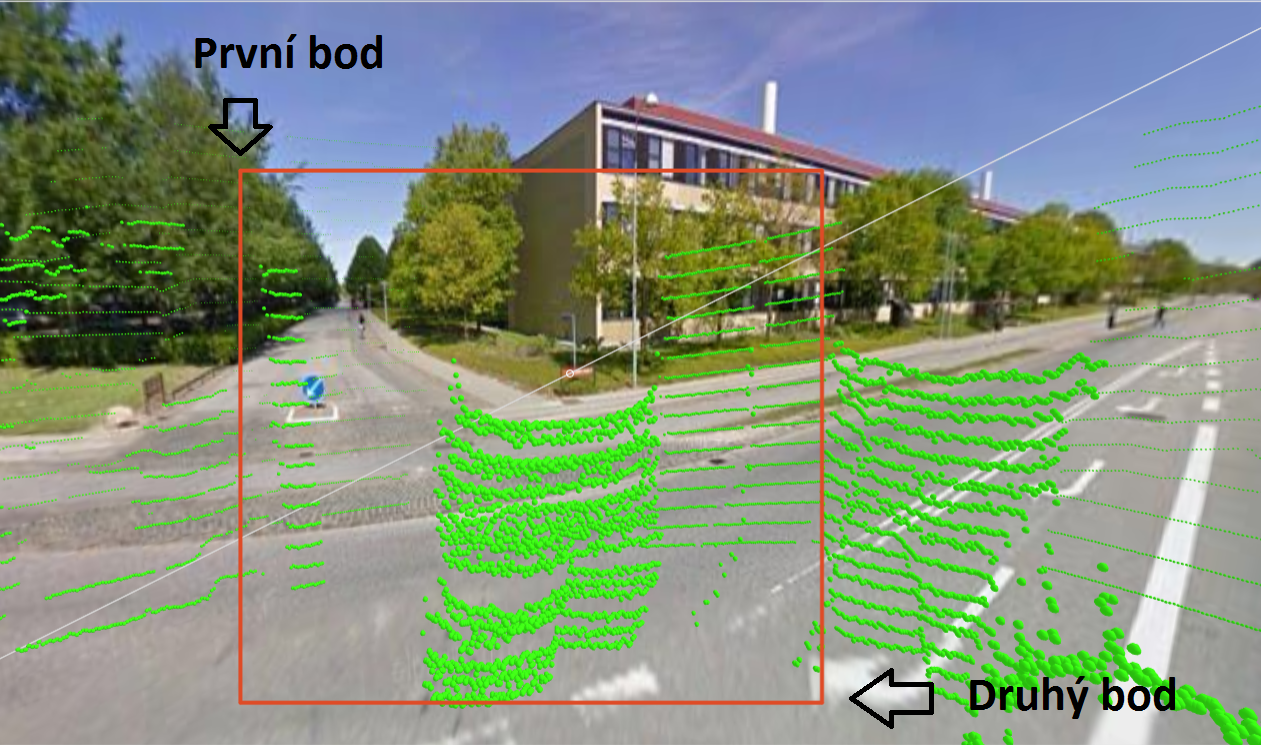
\includegraphics[width=\linewidth]{Figures/selectionBeforeProjection.png}
\caption{První bod a druhý bod selekce. }
\label{fig:selectionBefore}
\end{figure} 

\begin{figure}[H]
\centering
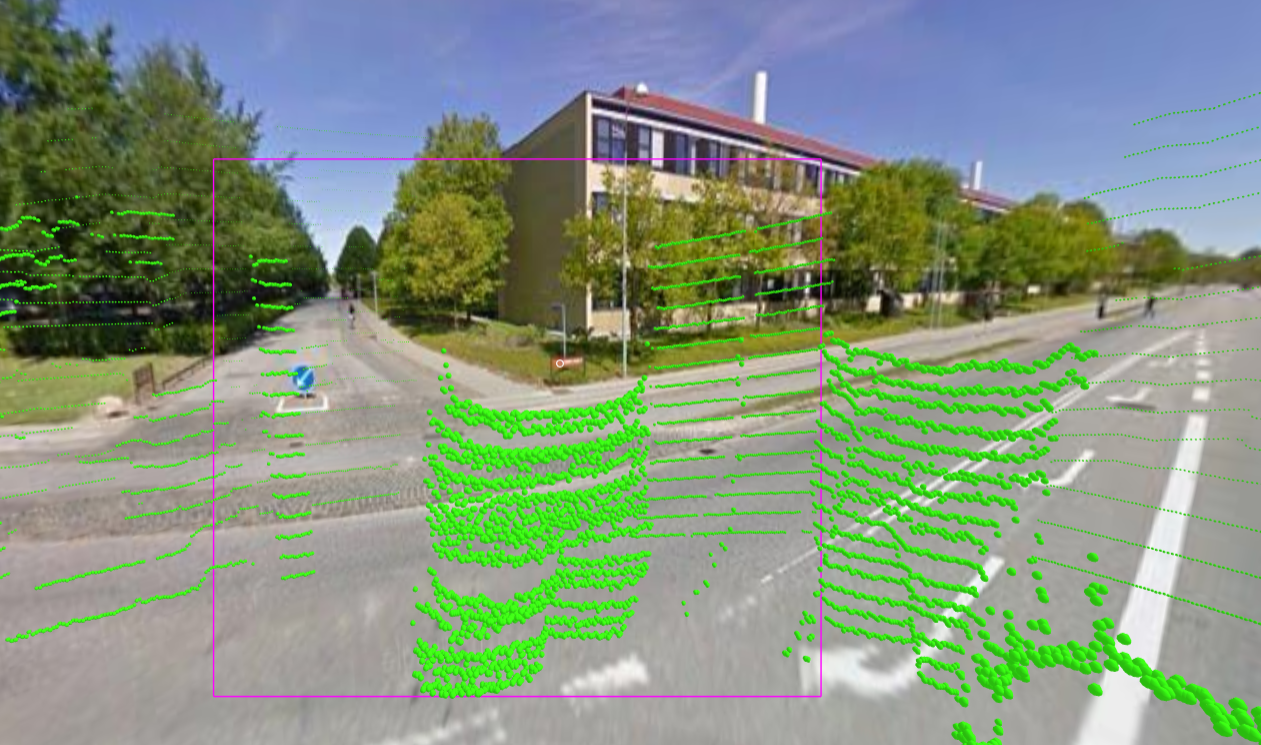
\includegraphics[width=\linewidth]{Figures/selectionAfterProjection.png}
\caption{Promítnutí bodů s již vytvořeným obrysem. }
\label{fig:selectionAfter}
\end{figure}

Zmíněné ukázky kódu nevytvářejí oranžový obrys \ref{fig:selectionBefore} na obrazovce. Již promítnutá selekce v prostoru \ref{fig:selectionAfter} je výsledkem z námi zmíněných ukázek kódu v kapitole \ref{secref:secref10}. Obrys \ref{fig:selectionBefore} nakreslený s pomocí canvas elementu na 2D obrazovce vypadá naprosto identicky, jako obrys v prostoru \ref{fig:selectionAfter} díky projekci.


\subsection{Zachycení obrazu selekce}\label{secref:secref13} 
Z kapitoly \ref{secref:secref16} jsme se dozvěděli základní princip perspektivní projekce, teď si ukážeme jakým způsobem je prováděna. K provedení projekce potřebujeme projekční matici. Každá kamera má projekční matici. Tato projekční matice 4x4 je vytvořena při vytvoření kamery. Nejdříve si vysvětlíme na základě jakých parametrů je perspektivní projekční matice vytvořena, poté si ukážeme výsledný tvar objektu po aplikování a nakonec implementaci zachycení obrazů selekcí. 

\begin{equation}
		P =
		\begin{bmatrix}%
    x & 0 & 0 & 0 \\
		0 & y & 0 & 0 \\ 
		0 & 0 & a & b \\
		0 & 0 & -1 & 0 
    \end{bmatrix}
\label{eq:eq4}
\end{equation}


 Zde můžeme vidět zjednodušený vzorec projekční matice kamery, kterou používá knihovna \texttt{Three.js}. Při vytváření nové kamery \ref{secr:additionalcamera} jsme specifikovali ještě další údaje. Tyto údaje jsou horizontální \texttt{FOV} ve stupních, poměr stran, vzdálenost přední a zadní roviny kamerového frustumu. Všechny tyto informace budeme potřebovat na vytvoření projekční matice. 

$$y = \frac{1}{\tan(\frac{FOV}{2} * \frac{\pi}{180})}$$ 

Tímto vzorcem vypočteme délku odvěsny uvnitř kamerového frustumu. Používáme funkci tangens s polovinou úhlu \texttt{FOV}, násobenou $\frac{\pi}{180}$ pro převod ze stupňů na radiány. Používáme pouze polovinu úhlu \texttt{FOV}, protože nás zajímá pravý úhel uvnitř frustumu. 

$$x = \frac{y}{aspect}$$ 

Pro získání této hodnoty využijeme výsledek předešlé rovnice a vydělíme ji poměrem stran. Tento poměr stran jsme získali při vytváření kamerového objektu. Tímto jsme upravili kamerové frustum tak, aby se nepodobalo pravidelnému rovnostrannému hranolu. Teď přední rovina kamerového frustumu již není čtverec, ale obdélník. Tyto dva parametry matice budou ovlivňovat hodnoty \texttt{x,y} v naší projekci. Hodnoty \texttt{a,b} budou ovlivňovat změnu měřítka objektu na vzdálenosti od pozice kamery. 

$$a = \frac{-\left(f+n\right)}{f-n}$$ 
$$b = \frac{-2fn}{f-n}$$ 

Výsledek hodnoty \texttt{a} bude měnit měřítko souřadnice \texttt{z} v kartézské soustavě souřadnic, a hodnota \texttt{b} bude konstanta, která bude přičtena k výsledné souřadnici \texttt{z}. Proměnná \texttt{f} nám značí vzdálenost od pozice kamery po nejvzdálenější rovinu kamerového frustumu. Tuto vzdálenost jsme vkládali při vytváření kamerového objektu. Proměnná \texttt{n} nám označuje vzdálenost k nejbližší rovině kamerového frustumu. 
% todo ask teacher why there is -1 : V rovnici \ref{eq:eq4} jste si mohli všimnout hodnoty $P_{32}=-1$ 

Ukážeme si, co se stane s objekty po aplikování projekční matice. Na obrázcích \ref{fig:projectionMatrixCameraFrustum1}, \ref{fig:projectionMatrixCameraFrustum2} vidíme modře zbarvené objekty uvnitř červeného kamerového frustumu. Červeně vyznačená část je jediná část scény, kterou jsme schopni vidět. Pokud vše vynásobíme projekční maticí, získáme \ref{fig:projectionMatrixCameraFrustum2}. Nyní se z našeho frustumu stal kvádr a všechny objekty byly také transformovány. Objekty, které jsou blíže kameře jsou větší, a s rostoucí vzdáleností se objekty stávají menšími. Stejně jako v reálném životě. Na obrázku \ref{fig:finalProjectionImageFromCamera} můžeme vidět vykreslení finálního výsledku. 

\begin{figure}[H]
    \centering
    \begin{minipage}[c]{0.48\linewidth}        %% or \columnwidth
        \centering
        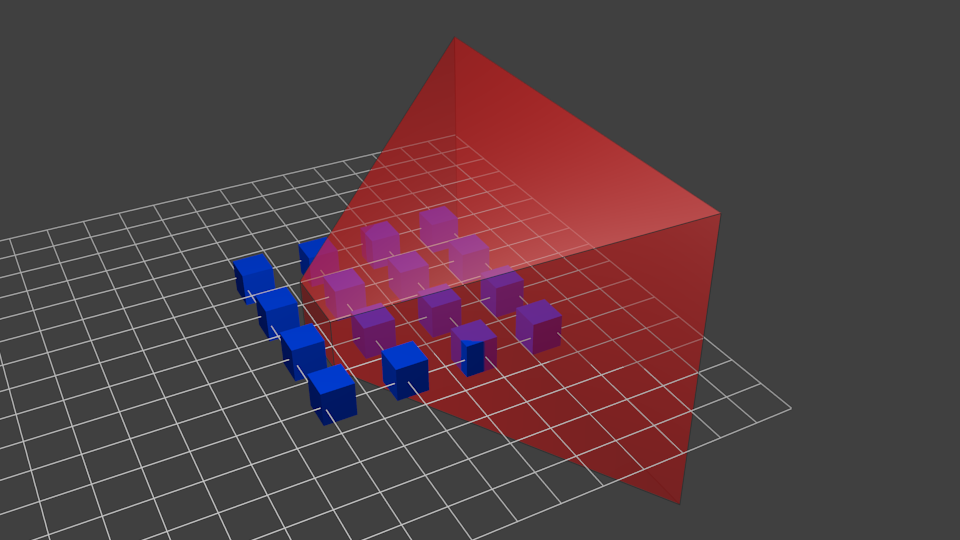
\includegraphics[width=\linewidth]{Figures/projectionMatrixCameraFrustum1.png}
        \caption{Ukázka kamerového frustumu před projekcí \cite{tutorial3matrices}.} % todo add citation http://www.opengl-tutorial.org/beginners-tutorials/tutorial-3-matrices/}
        \label{fig:projectionMatrixCameraFrustum1}
    \end{minipage}
    \begin{minipage}[c]{0.48\linewidth}        %% or \columnwidth
        \centering
        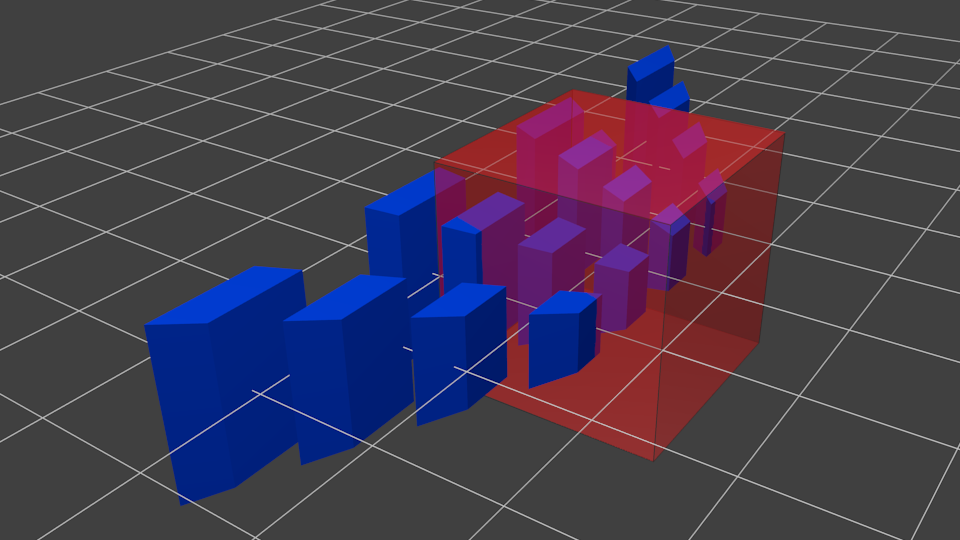
\includegraphics[width=\linewidth]{Figures/projectionMatrixCameraFrustum2.png}
        \caption{Ukázka kamerového frustumu po projekci \cite{tutorial3matrices}.}
        \label{fig:projectionMatrixCameraFrustum2}
    \end{minipage}
\end{figure}


\begin{figure}[H]
\centering
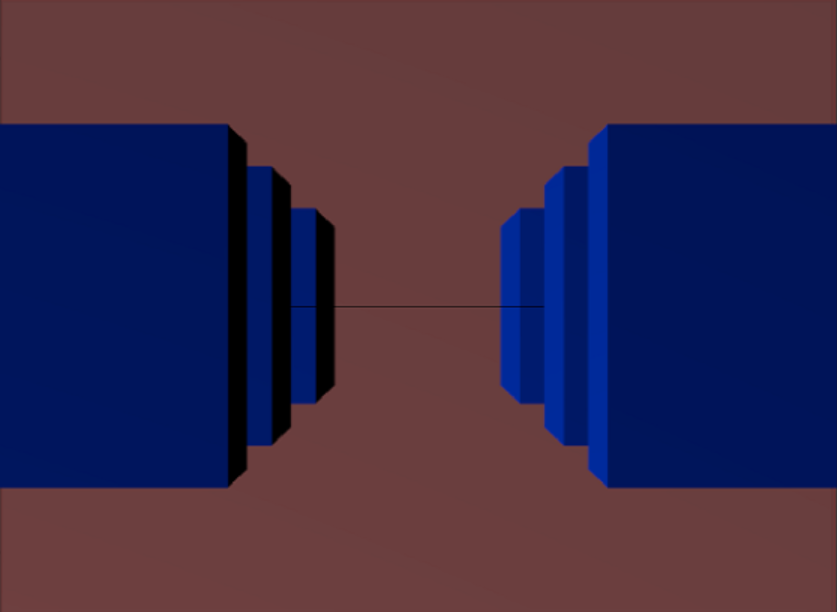
\includegraphics[width=0.6\linewidth]{Figures/finalProjectionImageFromCamera.png}
\caption{Výsledný obraz po projekci \cite{tutorial3matrices}. }
\label{fig:finalProjectionImageFromCamera}
\end{figure} 

K implementaci zachycení obrazu selekce budeme potřebovat novou kameru, která bude směřovat na střed naší selekce. Kameru potřebuje, aby nám vytvořila novou projekci. Vytvoříme si novou perspektivní kameru a namíříme na střed mezi dvěma námi vytvořenými body v podkapitole \ref{secref:secref10} 

\lstinputlisting[language=JavaScript,label={secr:additionalcamera},caption=Vytváření kamery pro sledování selekce.]{SourceCodes/additionalCamera.js}
 
Při vizualizování selekce také vytvoříme novou perspektivní kameru pro zachycení snímku selekce. Tento kód nám vytvoří novou perspektivní kameru a nastaví ji pozici ve středu scény. Dále ji nastavíme směr, na který se bude dívat. Vektoru s naším chtěným směrem docílíme tak, že sečteme vektor prvního a druhého bodu. Výsledkem je vektor procházející středem mezi těmito body. Nakonec přidáme naši kameru do skupiny pomocných kamer. 

\lstinputlisting[language=JavaScript,caption=Získání snímku z kamery.]{SourceCodes/createImageFromCameras.js}


\subsection{Export vybraných bodů z selekce}
Pro získání bodů v označené selekci si musíme uvědomit, že používáme perspektivní kameru a na monitoru vidíme projekci. Tím pádem obsah naší selekce bude připomínat jehlan, který má hlavní vrchol ve středu kamery a každá hrana obrysu leží na rovině procházející pozicí kamery. Roviny nám rozdělí prostor na požadovanou selekci. Tento prostor obsahuje všechny námi chtěné LIDARové body. Nejdříve musíme vytvořit naše roviny, abychom ohraničili náš prostor selekce. U našeho obrysu známe střední bod a délky stran. Pro vytvoření roviny jsou potřeba tři body neležící na jedné přímce. Jeden bod bude společný u všech rovin a tím bude pozice hlavní kamery. Další dva body budou vždy vrcholy hrany obrysu. Problém je, že známe pouze jediný bod, který není ovlivněn rotací. U zbylých bodů budeme muset vypočítat pozici po provedené rotaci. Obrys, který nemá žádnou rotaci, je vodorovný s osou \texttt{x}. 


\lstinputlisting[language=JavaScript,caption=Získání pozice vrcholu obrysu po provedení rotace.]{SourceCodes/rotateVectorAndReturnPosition.js} 


V ukázce chceme získat pravý spodní bod obrysu. Víme, že pozice obrysu je vždy ve středu. Abychom získali pravý spodní bod, tak musíme posunout středový bod selekce do středu scény a zrušit rotaci. Nyní na základě vzdálenosti \texttt{x} a \texttt{y} našeho obrysu vytvoříme vektor směřující k pravému dolnímu rohu obrysu bez rotace a s pozicí ve středu scény. Na tento vektor se použije stejná rotace, jako má náš obrys. Vysvětleme si, jak se rotace provede. Na rotaci se použijí transformační matice \eqref{eq:eq1}, \eqref{eq:eq2}, \eqref{eq:eq3} \cite{sojka_2003}.

\begin{equation}
		A_x =
		\begin{bmatrix}%
    1 & 0 & 0 \\
		0 & \cos \alpha & -\sin \alpha \\ 
		0 & \sin \alpha & \cos \alpha
    \end{bmatrix}
\label{eq:eq1}
\end{equation}

\begin{equation}
		A_y =
		\begin{bmatrix}%
    \cos \beta & 0 & \sin \beta \\
		0 & 1 & 0 \\ 
		-\sin \beta & 0 & \cos \beta
    \end{bmatrix}
\label{eq:eq2}
\end{equation}

\begin{equation}
		A_z =
		\begin{bmatrix}%
    \cos \gamma & -\sin \gamma & 0 \\
		\sin \gamma & \cos \gamma & 0 \\ 
		0 & 0 & 1
    \end{bmatrix}
\label{eq:eq3}
\end{equation}

Obrys má rotaci uloženou ve vlastnostech \texttt{x,y,z}, a každá z nich popisuje, o kolik radiánů se má otočit kolem stejnojmenné osy. Při zavolání metody \texttt{applyEuler()} na proměnné \texttt{vector} se nám tento vektor vynásobí maticí \eqref{eq:eq1}, kde $ \alpha = \texttt{line.rotation.x} $. Stejný postup se provede u \texttt{y} a \texttt{z}.  

Když máme všechny potřebné body po transformaci, tak vytvoříme naše roviny jehlanu. Musíme zajistit, aby normály všech rovin směřovali do ohraničeného prostoru. 

\lstinputlisting[language=JavaScript,caption=Získání všech bodů v selekci.]{SourceCodes/CustomFrustum.js} 

Třída \texttt{CustomFrustum} nám slouží pro uložení našeho jehlanu. Při sběru bodů selekce musíme v cyklu proiterovat všechny LIDARové body, a jestli jsou v našem jehlanu. Zjišťujeme, jestli vzdálenost od všech rovin je kladné číslo, pokud ne, tak víme, že bod leží mimo náš jehlan. Další, co si ke všem LIDARovým bodům uložíme, je náš obrys selekce z důvodu opětovnému přehraní dat ze selekcí.



\subsection{Pohyb selekcí} 
Než začneme, tak si musíme uvědomit, že naše obrysy jsou v prostoru scény a my se díváme na jejich projekci. Takže budeme muset zjistit za pomoci projekce na zadní rovinu frustumu kamery, jestli nějaký obrys byl protnut při této akci. Když zjistíme, že obrys byl zasáhnut, tak musíme získat všechny potřebné údaje pro budoucí práci s ním. Další se musíme rozhodnout, jakým způsobem chceme, aby se náš obrys pohyboval v trojrozměrném prostoru, a jakým způsobem budeme ovládat pohyb z dvojrozměrné obrazovky. Rozhodli jsme se, že naše obrysy musí být pohybovatelné okolo naší kamery a proto pohyb selekce musí kopírovat poloměr koule. Rotace obrysu bude záviset na hlavní kameře, ze které budeme pohyb ovládat.

\medskip
\begin{minipage}{\linewidth}
\lstinputlisting[language=JavaScript,label={secref:secref11},caption=Získání obrysu na základě události myši.]{SourceCodes/onMouseClickDrag.js} 
\end{minipage}

Budeme potřebovat vytvořit události na adekvátní akce myši. K tomu budeme potřebovat použít \texttt{THREE.Raycaster}, který nám pomoci bodu z naší obrazovky zjistí, zda nějaký objekt je ve scéně za touto projekcí. Nejdříve nastavíme \texttt{raycaster}, aby použil projekční matici naší hlavní perspektivní kamery, pak použijeme metodu \texttt{intersectObjects} s parametrem \texttt{objects}, ten obsahuje všechny naše obrysy. Pokud nějaký obrys našel, tak si náš objekt uložíme do třídní proměnné \texttt{selected}. Kdyby bylo více obrysů za sebou, metoda by vrátila oba obrysy, ale seřadila by je od nejbližšího po nejvzdálenější. Proměnnou \texttt{selected} použijeme i při dalších událostech, pak pomocí metody \texttt{intersectSphere} získáme pozici střetu koule, po které chceme obrys pohybovat s projekčním paprskem. Výsledek je pak uložen do proměnné \texttt{intersection}. Obrys má pouze jediný pevný bod, na který se nevztahuje rotace, a ten je uložen ve vlastnosti \texttt{position}. Od tohoto bodu je vytvořená geometrie, která podléhá rotaci. Když budeme vybírat obrys v naší scéně, tak nebudeme vždy mířit na tento bod, proto potřebuje odchylku našeho kliknutí od pevného bodu. To nám zařizuje proměnná \texttt{offset}, která zkopíruje bod dotyku s koulí a odečte z něj pozici pevného bodu obrysu. Výsledkem bude vektor, který při pohybu budeme muset odčítat, abychom mohli z jakéhokoliv místa pohybovat obrysem a zachovali pohyb po chtěné kouli. Kód \ref{secref:secref11} přiřadíme k události \texttt{mousedown}.

\lstinputlisting[language=JavaScript,label={secref:secref12},caption=Pohyb obrysu ve scéně.]{SourceCodes/onMouseMoveDrag.js}

Do proměnné \texttt{rect} získáme velikosti naší scény v prohlížeči a nastavíme \texttt{raycaster}, aby směřoval na pozici v prostoru, kterou získáme projekcí aktuální pozice z obrazovky. Stejně jako v předchozím příkladu použijeme proměnnou \texttt{intersection} pro získání pozice střetu s koulí po projekci našeho kurzoru na kouli, a nastavíme délku tohoto vektoru na poloměr koule. Nakonec nastavíme obrysu rotaci na základě kamery, aby obrys měl rotaci proti kameře. Tento kód \ref{secref:secref12} přiřadíme k události \texttt{mousemove}.    

\lstinputlisting[language=JavaScript,label={secref:secref14},caption=Zrušení pohybu a zaměření kamery pro zasílání obrázových dat.]{SourceCodes/onMouseCancelDrag.js}

Při událostech typu \texttt{mouseup, mouseleave} nesmíme zapomenout natočit kameru, kterou zachycujeme obrazová data selekcí \ref{secref:secref13}. Musíme zjistit bod ve středu obrysu, na který byla použita rotační transformace. K tomu vytvoříme vektor, který bude popisovat směr ke středu obrysu bez rotace. Nasledně na tento vektor aplikujeme kompletní rotaci stejnou jako je na obrysu a přičteme k němu jeho pevný bod. Získáme pozici středu obrysu a nyní jen kameru sledující selekci nastavíme, aby sledovala tuto pozici pomocí metody \texttt{lookAt}. Nakonec vyprázdníme proměnnou \texttt{selected}. Tyto části kódu nám zařídí, že naše bude pohybovatelná okolo naší kamery při zachování dosavadní funkcionality systému.


\section{Závěr}
Cílem bakalářské práce bylo nastudovat potřebné webové knihovny pro vytvoření vizualizačního nástroje LIDARových dat s podporou selekcí obrazových i datových částí. Součástí bylo nastudování principu LIDARu, ukládání a formát jeho dat. Tato část byla nutná k vizualizování LIDARových dat.

V rámci této práce byla vytvořena vizualizace LIDARových dat ve webovém prohlížeči s podporou selekcí částí prostoru. Selekce jsou na základě akcí upravovatelné. Export LIDARových bodů selekce na server plus obrazová data pozadí těchto bodů. Znovupřehrání selekcí i s obsaženými daty také zaimplementováno.

Tato práce mi byla velkým přínosem. Rozšířila mi obzor, a díky ní jsem získal obecný přehled ohledně počítačové grafiky, vizualizačních algoritmů a nepostradatelnou součást matematiky. Délka implementace systému se velmi lišila od mých odhadů z důvodu neznalosti základů geometrii, projekcí kamer, transformačních matic a nulových zkušeností s WebGl. I s brzkým začátkem implementační části projektu se z již zmíněných důvodů produktivní vývoj blížil až ke konci projektu.
 
%\addcontentsline{toc}{section}{Závěr}

\newpage
\nocite{*}
\renewcommand\refname{Literatura}
%\section*{Literatura}
\addcontentsline{toc}{section}{Literatura}

%\bibliography{mybib}
%\bibliographystyle{plain}
\printbibliography
%\bibliography{mybib}


%add to citation https://developer.okta.com/blog/2019/07/19/mysql-vs-postgres


% https://en.wikipedia.org/wiki/OpenGL
% https://en.wikipedia.org/wiki/JavaScript
% https://en.wikipedia.org/wiki/List_of_WebGL_frameworks
% https://en.wikipedia.org/wiki/WebGL
% https://cs.wikipedia.org/wiki/JavaScript
% https://en.wikipedia.org/wiki/Point_cloud
% 	
%		
%https://aframe.io/docs/0.9.0/introduction/html-and-primitives.html#sidebar
%
%https://www.scratchapixel.com/lessons/3d-basic-rendering/rendering-3d-scene-overview/visibility-problem
\end{document}